\documentclass[../Main.tex]{subfiles}
\begin{document}

\subsection{Introduction}

Multi-Agent Reinforcement Learning (MARL) extends the standard Reinforcement Learning (RL) paradigm to environments involving multiple interacting agents \cite{busoniu2008comprehensive}. Each agent learns from experience and interacts with the environment, which now includes other learning agents. The outcome of each agent’s actions depends not only on the environment dynamics but also on the behavior of the other agents. This extended agent-environment interaction is visualized in Figure~\ref{fig:marl_interaction_loop}.


\begin{figure}[H]
    \centering
    \includegraphics[width=0.5\linewidth]{marl-framework.png}
    \caption{The general interaction loop in a multi-agent system. Each agent sends an action to the system (environment) and receives back a shared state and an individual reward.}
    \label{fig:marl_interaction_loop}
\end{figure}

Based on the relationship between agent rewards, MARL problems are typically classified into three categories:
\begin{itemize}
    \item \textbf{Pure Competition}: Modeled as zero-sum games where agents' rewards are in direct conflict. For example, in Chess or Poker, \( R_1(s, a_1, a_2) = - R_2(s, a_1, a_2) \).
    \item \textbf{Pure Cooperation}: All agents share the same reward signal, i.e., \( R_1 = R_2 = \dots = R_N \). Examples include cooperative navigation or collaborative target acquisition.
    \item \textbf{Mixed-Sum}: A combination of cooperation and competition. A common example is autonomous driving, where vehicles collaborate for traffic flow but also compete for space and efficiency.
\end{itemize}

\subsection{Pure Cooperative Settings}

In fully cooperative multi-agent environments, all agents aim to optimize a shared objective. The corresponding framework is called the \textbf{Decentralized Partially Observable Markov Decision Process (Dec-POMDP)} \cite{oliehoek2016concise}.

A Dec-POMDP is defined by the tuple:
\[
(S, \{A_i\}_{i=1}^n, T, R, \{\Omega_i\}_{i=1}^n, O, \gamma)
\]
with:
\begin{itemize}
    \item \( S \): global state space.
    \item \( A_i \): action space of agent \( i \); joint action space \( A = A_1 \times \cdots \times A_n \).
    \item \( T(s, a, s') = \Pr(s'|s, a) \): transition function.
    \item \( R(s, a) \): shared reward function.
    \item \( \Omega_i \): observation space for agent \( i \); joint observation space \( \Omega = \Omega_1 \times \cdots \times \Omega_n \).
    \item \( O(s', a, o) = \Pr(o \mid s', a) \): observation function.
    \item \( \gamma \): discount factor.
\end{itemize}

Each agent \( i \) maintains a local action-observation history:
\[
\tau_i = (o^i_1, a^i_1, o^i_2, \dots, o^i_t)
\]

\begin{figure}[H]
    \centering
    \includegraphics[width=0.75\linewidth]{img/full-cooperation.png}
    \caption{Cooperative MARL as a Dec-POMDP. All agents optimize a joint reward signal.}
\end{figure}


\subsection{Learning Paradigms in MARL}

There are three principal training and execution paradigms in multi-agent reinforcement learning \cite{oroojlooy2023review}:

\begin{itemize}
    \item \textbf{Decentralized Training and Execution (DTE)}: Each agent is trained and deployed independently, based only on its local information.
    \item \textbf{Centralized Training and Execution (CTE)}: A centralized controller observes the full environment and controls all agents directly.
    \item \textbf{Centralized Training, Decentralized Execution (CTDE)}: During training, agents can access global information (including other agents' observations and actions), but during execution, they act independently based only on local observations.
\end{itemize}

\begin{figure}[h]
\centering
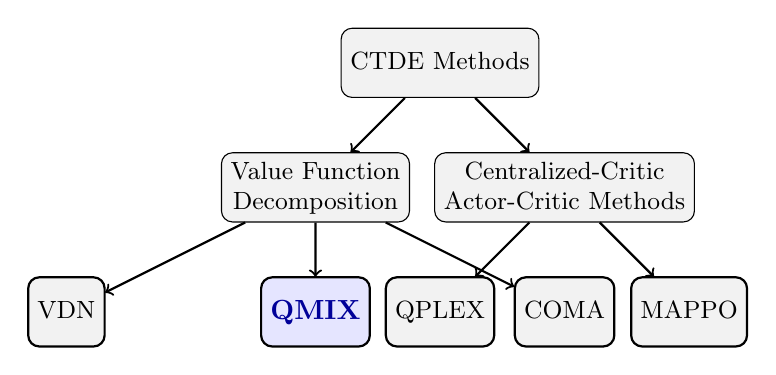
\begin{tikzpicture}[
    level distance=4.5em,
    sibling distance=9em,
    every node/.style={font=\small, align=center, rounded corners, draw=black, fill=gray!10, minimum height=2.5em, text depth=0.25ex},
    edge from parent/.style={draw, ->, thick}
]
\node (root) {CTDE Methods}
    child { node {Value Function\\ Decomposition}
        child { node {VDN} }
        child { node[fill=blue!10, text=blue!60!black, font=\bfseries] {QMIX} }
        child { node {COMA} }
    }
    child { node {Centralized-Critic\\ Actor-Critic Methods}
        child { node {QPLEX} }
        child { node {MAPPO} }
    };
\end{tikzpicture}
\caption{Taxonomy of Centralized Training with Decentralized Execution (CTDE) methods. QMIX is a value decomposition method.}
\label{fig:ctde-taxonomy}
\end{figure}

\section{QMIX}

\subsection{Value Function Factorization Methods}

In cooperative multi-agent reinforcement learning, a common challenge is learning a value function that supports decentralized execution while leveraging centralized training. Early methods aimed to learn a joint Q-function but faced difficulties with scalability and coordination.

\begin{itemize}
    \item \textbf{Modern Approach:} Each agent \(a\) learns a local Q-function \(Q_a(\tau_a, u_a)\) based on its action-observation history \(\tau_a\), and a mixing function is used to approximate the joint Q-function \(Q_{\text{tot}}(\tau, \mathbf{u})\).
    \item \textbf{Decentralized Execution:} At test time, each agent selects actions greedily with respect to its local Q-function. The mixing function must ensure consistency between local argmax actions and global optimality.
\end{itemize}

\begin{quote}
\textbf{Note:} We use the notation \( a \) for agents, \( u = (u_1, u_2, \dots, u_n) \) for joint actions, and \( \tau_a \) for agent \(a\)'s history.
\end{quote}

\subsection{VDN: Value Decomposition Networks}

Value Decomposition Networks (VDN) propose a simple linear factorization of the joint Q-function \cite{sunehag2017value}:
\[
Q_{\text{tot}}(\tau, u) \approx \sum_{a=1}^{N} Q_a(\tau_a, u_a)
\]
\begin{itemize}
    \item Each agent independently learns a local Q-function \(Q_a\) from its partial trajectory \(\tau_a\).
    \item Centralized training is possible with joint experiences.
    \item At execution, each agent acts independently by selecting \( \arg\max_{u_a} Q_a(\tau_a, u_a) \).
\end{itemize}

\begin{exampleblock}{Motivation for Generalization}
    VDN lacks the ability to model interaction between agents because:
    \begin{itemize}
        \item It ignores global state information in the mixing process.
        \item It fails in tasks requiring complex coordination.
    \end{itemize}
\end{exampleblock}

\subsection{From VDN to Monotonic Factorizations}

VDN assumes linearity. QMIX generalizes this to a broader class of \textbf{monotonic functions} \cite{rashid2018qmix}:
\[
\arg\max_{\mathbf{u}} Q_{\text{tot}}(\tau, \mathbf{u}) = 
\Bigl(
\arg\max_{u_1} Q_1(\tau_1, u_1), \dots,
\arg\max_{u_n} Q_n(\tau_n, u_n)
\Bigr)
\]
This guarantees that the global greedy action can be decomposed into local greedy actions — crucial for decentralized execution.

\subsection{Monotonicity and QMIX}

QMIX ensures that \( Q_{\text{tot}} \) is monotonic in each local Q-value:
\[
\frac{\partial Q_{\text{tot}}}{\partial Q_a} \geq 0 \quad \forall a
\]
To achieve this:
\begin{itemize}
    \item A \textbf{mixing network} is used to combine the local Q-values into a global one.
    \item \textbf{State-dependent weights} are produced by \textbf{hypernetworks} to allow context-aware combination, while preserving monotonicity.
\end{itemize}

\subsection{QMIX Architecture}
\begin{figure}[h]
    \centering
    \includegraphics[width=\linewidth]{img/qmix.png}
    \caption{QMIX architecture. Hypernetworks (red) generate state-dependent weights for the mixing network (blue).}
\end{figure}

\begin{itemize}
    \item \textbf{Agent Networks:} Each agent learns \( Q_a(\tau_a, u_a) \) using a recurrent neural network (e.g., GRU or LSTM).
    \item \textbf{Mixing Network:} Takes the vector \( \mathbf{q} = [Q_1, \dots, Q_N] \) as input and outputs \( Q_{\text{tot}} \).
    \item \textbf{Hypernetworks:} Generate the mixing network’s weights and biases as functions of the global state \(s\).
\end{itemize}

\subsection{Hypernetworks}

A \textbf{hypernetwork} is a neural network designed to generate the weights and biases of another network — often referred to as the \emph{target network} \cite{ha2016hypernetworks}. In the context of QMIX, hypernetworks take the global state as input and produce the parameters (weights and biases) for the mixing network that combines the individual agent Q-values. This mechanism allows the mixing function to be \textbf{state-dependent} while still satisfying the \textbf{monotonicity constraint}, which is crucial for enabling decentralized execution. By learning how to generate these parameters based on the state, hypernetworks enable flexible yet structured coordination among agents, adapting the value composition strategy to different parts of the state space without violating the factorization conditions.

\begin{figure}[h]
    \centering
    \includegraphics[width=\linewidth]{img/hypernetwork.png}
    \caption{A hypernetwork generates the parameters of another neural network — here, used to compute state-conditioned mixing weights.}
\end{figure}

\subsection{Training Objective}

QMIX follows a standard Q-learning loss using target networks:
\[
y = r + \gamma \max_{\mathbf{u}'} Q_{\text{tot}}(\tau', u', s';\ \theta^-)
\]
\[
\mathcal{L}(\theta) = \mathbb{E} \left[ \left( Q_{\text{tot}}(s, \mathbf{u}; \theta) - y \right)^2 \right]
\]
Here, \( \theta^- \) are target network parameters, and due to monotonicity, the max operator distributes over agents.

\subsection{Mixing Network Equation}
\[
Q_{\text{tot}}(\tau, u, s;\ \theta) = W_2(s)^\top \,\sigma\!\Big(W_1(s)\,\mathbf{q} + b_1(s)\Big) + b_2(s)
\]
\begin{itemize}
    \item \( \mathbf{q} = [Q_1, \dots, Q_N]^\top \)
    \item \( W_1(s), W_2(s), b_1(s), b_2(s) \): state-dependent weights and biases from hypernetworks.
    \item \( \sigma(\cdot) \): non-linear activation (e.g., ELU).
\end{itemize}

\subsection{Agent Networks}

Each agent’s utility function is:
\[
Q_a(\tau_a, u_a) = \text{RNN}_\theta(\tau_a)
\]
\begin{itemize}
    \item Handles partial observability with recurrent architecture (e.g., GRU).
    \item Outputs a vector of size \( |\mathcal{A}_a| \).
\end{itemize}

\textbf{Execution:}
\begin{itemize}
    \item Each agent selects \( \arg\max_{u_a} Q_a(\tau_a, u_a) \).
    \item Coordination emerges from the monotonic structure learned during centralized training.
\end{itemize}

\section{Results}

To evaluate the performance of QMIX against baseline methods, we compare it with Independent Q-Learning (IQL) and Value Decomposition Networks (VDN) on both synthetic and real multi-agent benchmarks. The following results highlight the expressiveness and coordination capabilities of QMIX in cooperative settings \cite{rashid2018qmix}.

\subsection{Two-Step Game}

The two-step game is a simple matrix game designed to test an algorithm’s ability to model joint action values and execute coordinated behavior.

\begin{figure}[h]
    \centering
    \includegraphics[width=0.8\linewidth]{img/2step-game.png}
    \caption{Payoff matrices in the two-step game. Agent 1’s first action (A or B) determines the state transition to either 2A or 2B.}
    \label{fig:2step-matrix}
\end{figure}

\subsection{State-Value Estimation}

We evaluate how accurately VDN and QMIX can model the joint value function \( Q_{\text{tot}} \). The results show that QMIX captures the correct state-action dependencies, while VDN tends to oversimplify due to its linear summation.

\begin{figure}[h]
    \centering
    \includegraphics[width=0.8\linewidth]{img/results/2step-game-results.png}
    \caption{Estimated \( Q_{\text{tot}} \) in the two-step game for (a) VDN and (b) QMIX.}
    \label{fig:2step-results}
\end{figure}

\subsection{StarCraft II Micromanagement Benchmark}

A more realistic benchmark is provided by the StarCraft II micromanagement environment, where agents (units) must coordinate to defeat enemy forces across several maps. Win rates over six different scenarios demonstrate that QMIX significantly outperforms both IQL and VDN, particularly in scenarios requiring tight coordination. I will further explain the SMAC environment in a later section.

\begin{figure}[h]
    \centering
    \includegraphics[width=\linewidth]{img/results/abblations.png}
    \caption{Win rates of IQL, VDN, and QMIX on six StarCraft II combat scenarios. Dashed line indicates heuristic baseline.}
    \label{fig:starcraft}
\end{figure}

\subsection{Ablation Studies}

To better understand the contribution of each architectural component in QMIX, several ablation variants were evaluated:
\begin{itemize}
    \item \textbf{QMIX-NS}: QMIX without state-dependent mixing.
    \item \textbf{QMIX-Lin}: QMIX using a linear mixing function.
    \item \textbf{VDN-S}: VDN extended with state information in mixing.
\end{itemize}

\begin{figure}[h]
    \centering
    \includegraphics[width=1\linewidth]{img/results/abblations.png}
    \caption{Win rates for QMIX and its ablations on three StarCraft II maps: 3m, 2s\_3z, and 3s\_5z.}
    \label{fig:abblations}
\end{figure}

The results confirm that both state information and non-linear mixing functions are critical to QMIX’s superior performance. Notably, even the addition of state information to VDN (VDN-S) does not match the expressiveness achieved by QMIX.

\section*{Conclusion}
\addcontentsline{toc}{section}{Conclusion}

This chapter has systematically constructed the theoretical framework necessary to understand the contributions of this project. We began by laying the foundations of single-agent Reinforcement Learning, defining the mathematical formalisms and core concepts that govern learning from interaction. We then surveyed the evolution of solution methods, from tabular algorithms to the deep function approximation techniques of Deep Q-Learning that enable scaling to complex problems.

Culminating this theoretical journey, we extended our focus to the multi-agent cooperative setting, introducing the Centralized Training with Decentralized Execution paradigm and providing a detailed analysis of the QMIX algorithm. Equipped with this comprehensive theoretical foundation, we are now prepared to transition from theory to practice. The following chapter will detail our novel experimental work, which builds directly upon the principles and challenges outlined here.

\clearpage
\biblio % Needed for referencing to working when compiling individual subfiles - Do not remove
\end{document}